\section{Introduction}

Deformable object manipulation has long been a challenging topic in the field of robotic manipulation~\citep{sanchez2018robotic,yin2021modeling,zhu2022challenges,hoang2025geometryaware,zhao2025learning,wangdexgarmentlab,huang2026soma,li2026lehome}.
Among the diverse forms of common deformable materials, deformable linear objects (DLOs), such as wires and ropes in~\Cref{fig:teaser}(a), exhibit unique features and properties. Compared to volumetric materials, a DLO can be represented by a relatively small set of vertices and degrees of freedom due to its linear co-dimensional nature. However, this apparent simplicity does not make manipulation any easier. Manipulating deformable linear objects (DLOs) presents several unique challenges: (1) high precision is essential due to the co-dimensional nature of these objects, (2) DLOs have complex dynamics and varied topologies that are challenging to model, and (3) perception algorithms often find it difficult to accurately detect the state of DLOs, especially when self-crossings happen.

Prior work has addressed DLO manipulation in several directions. (1) Approaches focusing on perception, such as cable-tracing tasks~\citep{caporali2022ariadne+, kicki2023dloftbs, shivakumar2022sgtm, viswanath2023handloom, luo2025tsl,dinkel2025dlo}, which require extensive data collection and rely heavily on synthetic datasets for training. (2) Approaches focusing on manipulation, such as cable untangling~\citep{viswanath2021disentangling, sundaresan2021untangling} and shape control~\citep{yu2022global,yu2022shape,caporali2024deformable,gu2025learning}, which generally target specific tasks and are difficult to generalize to other DLO-related problems. From this perspective, we argue that a simulation and benchmark platform for DLO manipulation is necessary—both for generating perception training data and for facilitating policy learning for manipulation.

\begin{figure*}[t]
    \centering
    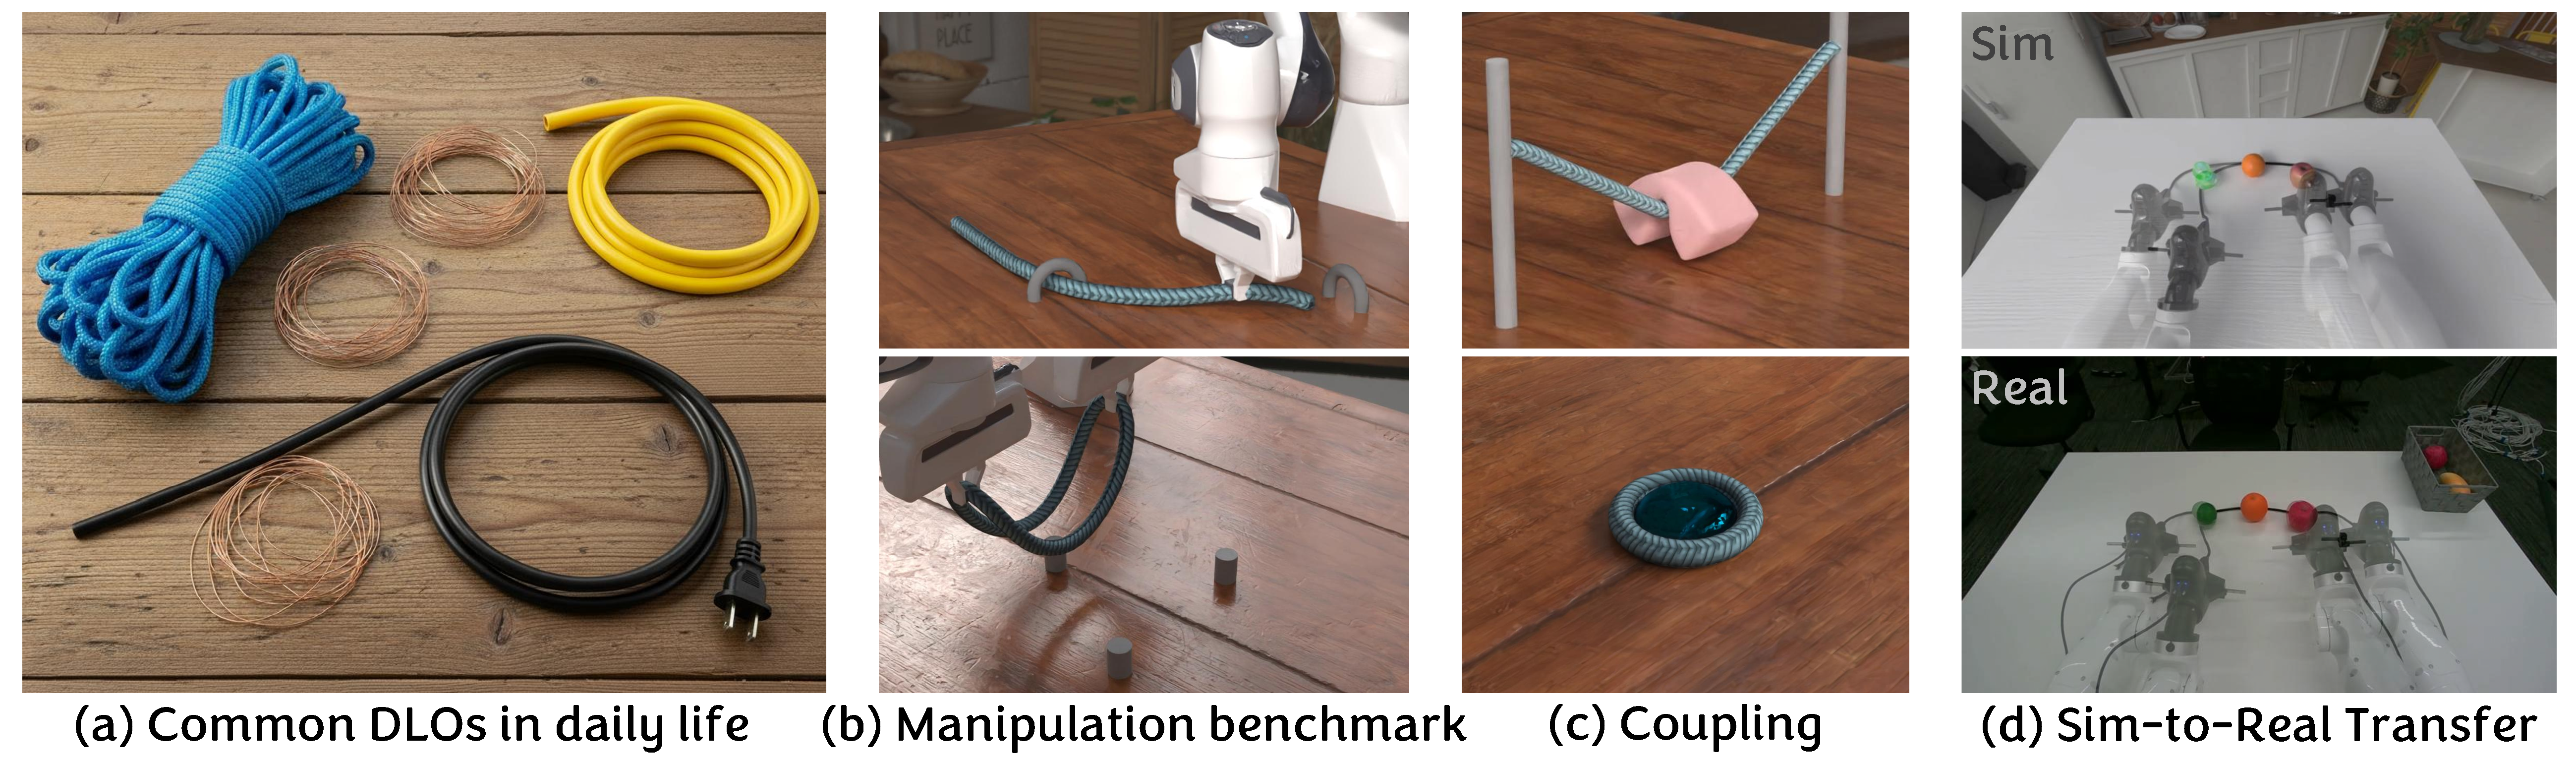
\includegraphics[width=\linewidth]{figs/teaser_v1.pdf}
    \vspace{-6mm}
    \caption{\textbf{DLO-Lab.} (a) We encounter various deformable linear objects (DLOs) in our daily life, such as cables, ropes, and wires. (b) To facilitate versatile robotic skill learning for DLOs with diverse material properties, we introduce \emph{DLO-Lab}, a differentiable simulation environment for DLOs with a set of benchmark tasks. (c) Our simulator effectively supports coupling with other materials, enabling the interaction between DLOs and other objects. (d) We also conduct real-world experiments to deploy a trained policy.}
    \label{fig:teaser}
\end{figure*}

Several prior works have proposed simulations for modeling DLO dynamics~\citep{lin2021softgym,naughton2021elastica,li2021codimensional,tong2023fully,chendifferentiable,jiang2025phystwin}. However, as shown in~\Cref{tab:feature-comparison}, each of them only supports a subset of the desired features. Among these features, coupling and differentiability are the two most important properties to enable flexible manipulation and efficient policy optimization. 
On one hand, coupling effectively models the physical interactions between DLOs, robot manipulators, and other objects in the scene. This physical fidelity is the foundation for simulating a wide range of complex, contact-rich manipulation tasks.
On the other hand, differentiability is crucial for efficient policy optimization. It provides gradient information of the system's dynamics, which quantifies how changes in the robot's actions influence the final state of the DLO.
However, none of the previous studies address \emph{both} coupling and differentiability, and they also overlook other common properties found in DLOs, such as bending plasticity and loop topology.
Therefore, we identify the need for a simulation environment that integrates diverse material couplers and is tailored for robotic skill acquisition in various DLO manipulation tasks.

To this end, we propose a differentiable simulation engine, DLO-Lab, featuring diverse material behaviors of DLOs and their interactions with other entities. Building upon the Genesis platform~\citep{Genesis}, we implement a customized solver for DLOs and their coupling with various materials, including rigid bodies, elastic and plastic objects, fluids, and beyond. Most operators in our solver are naturally differentiable by leveraging Taichi~\citep{hu2019taichi,hu2020difftaichi} as the programming language. Specifically, our DLO solver primarily follows the Discrete Elastic Rods (DER) theory~\citep {bergou2008discrete,bergou2010discrete}, enhanced with bending plasticity, support for loop topologies, and heterogeneous material composition. In addition, we implement frictional contact between DLOs and other materials and ensure that the differentiability requirement is satisfied during contact. As a result, our simulation is able to simulate the coupling between DLOs with other materials supported by Genesis, such as fluids and elastic objects, as shown in~\Cref{fig:teaser}(c).

Based on this simulation environment, we design a set of benchmark tasks that highlight the properties and capabilities of DLOs. Many of these tasks mimic practical applications like cable routing, wire forming, and unknotting, which are inherently long-horizon and constrained by topology. In such scenarios, the success of a task also depends on identifying suitable grasping points and implementing strategic re-grasping, making simple end-to-end policy learning impractical.
To tackle these challenges, we propose a specialized DLO agent that offers structural guidance through two main capabilities: (1) grasp proposal, which identifies optimal interaction points to maximize control authority, and (2) task decomposition, which breaks down complex objectives into manageable subtasks. We evaluate various algorithms on the benchmark tasks, including model-free reinforcement learning (MFRL) methods~\citep{schulman2017proximal,haarnoja2018soft}, first-order model-based reinforcement learning (FO-MBRL) methods~\citep{xingstabilizing,xuaccelerated}, and sample- or gradient-based trajectory optimization~\citep{cmaes}. 

Our experiments suggest that gradient-based methods achieve the highest sample efficiency when informative gradients are available, demonstrating the clear advantage of differentiable simulation. However, for tasks characterized by discontinuous contact dynamics or sparse rewards, sampling-based trajectory optimization proves more robust. We further observe that learning generalizable closed-loop policies remains significantly more sample-intensive than optimizing open-loop trajectories. Finally, real-world validation, \eg,~\Cref{fig:teaser}(d), confirms that policies optimized in our simulator can be effectively transferred to physical hardware, successfully bridging the sim-to-real gap.

\begin{table*}[t]
\begin{center}
\setlength{\tabcolsep}{1.2mm}{
\begin{tabular}{ccccccc}
\toprule
\textbf{Simulators}  & \textbf{Solver}       & \textbf{Elastic Potentials} & \textbf{Bending Plasticity} & \textbf{Loop Topology} & \textbf{Coupling} & \textbf{Differtiability}  \\
\midrule
Bi-LSTM & NN & & & & & \checkmark \\
GNN & NN & & & & & \checkmark \\
XPBD & PBD & & & & & \checkmark \\
SoftGym & PBD & & & & \checkmark & \\
Elastica & Cosserat Rods  & \checkmark & & & \checkmark &\\
C-IPC & DER & \checkmark & & & \checkmark & \\
IMC & DER & \checkmark & & & & \\
DaXBench & MPM & \checkmark & & & & \checkmark \\
DEFORM & NN & \checkmark & & & & \checkmark \\
PhysTwin & Spring-Mass & \checkmark & & & & \checkmark \\
\hline
Ours & Customized & \checkmark & \checkmark & \checkmark & \checkmark & \checkmark \\
\bottomrule
\end{tabular}
}
\caption{\textbf{Comparison with existing simulators for DLOs.} ``NN'' refers to neural networks. ``DER'' refers to the Discrete Elastic Rods~\citep{bergou2008discrete,bergou2010discrete} theory. ``Coupling'' refers to interaction between DLOs and other materials (\eg, rigid or soft bodies).}
\label{tab:feature-comparison}
\end{center}
\vspace{-6mm}
\end{table*}

We summarize our main contributions as follows:
\begin{itemize}[align=right,itemindent=0em,labelsep=2pt,labelwidth=1em,leftmargin=*,itemsep=0em] 
    \item We propose a differentiable simulation engine for DLOs and their interactions with different materials. Our simulation environment supports various material configurations and provides a standardized interface for both RL- and gradient-based policy learning algorithms.
    \item We introduce DLO-Lab, a comprehensive benchmark for robotic manipulation with DLOs. This benchmark aims to facilitate the exploration of versatile manipulation skills across a diverse set of DLOs. Based on DLO-Lab, we analyze the performance of sampling- and gradient-based policy learning methods and the challenges they encounter.
    \item We design a specialized agent for DLO manipulation tasks. It facilitates long-horizon manipulation by automatically decomposing complex tasks into executable sub-stages and proposing optimal grasping points to maximize control authority over the DLOs.
\end{itemize}
